\chapter{支架}
\begin{figure}[htbp]
\centering
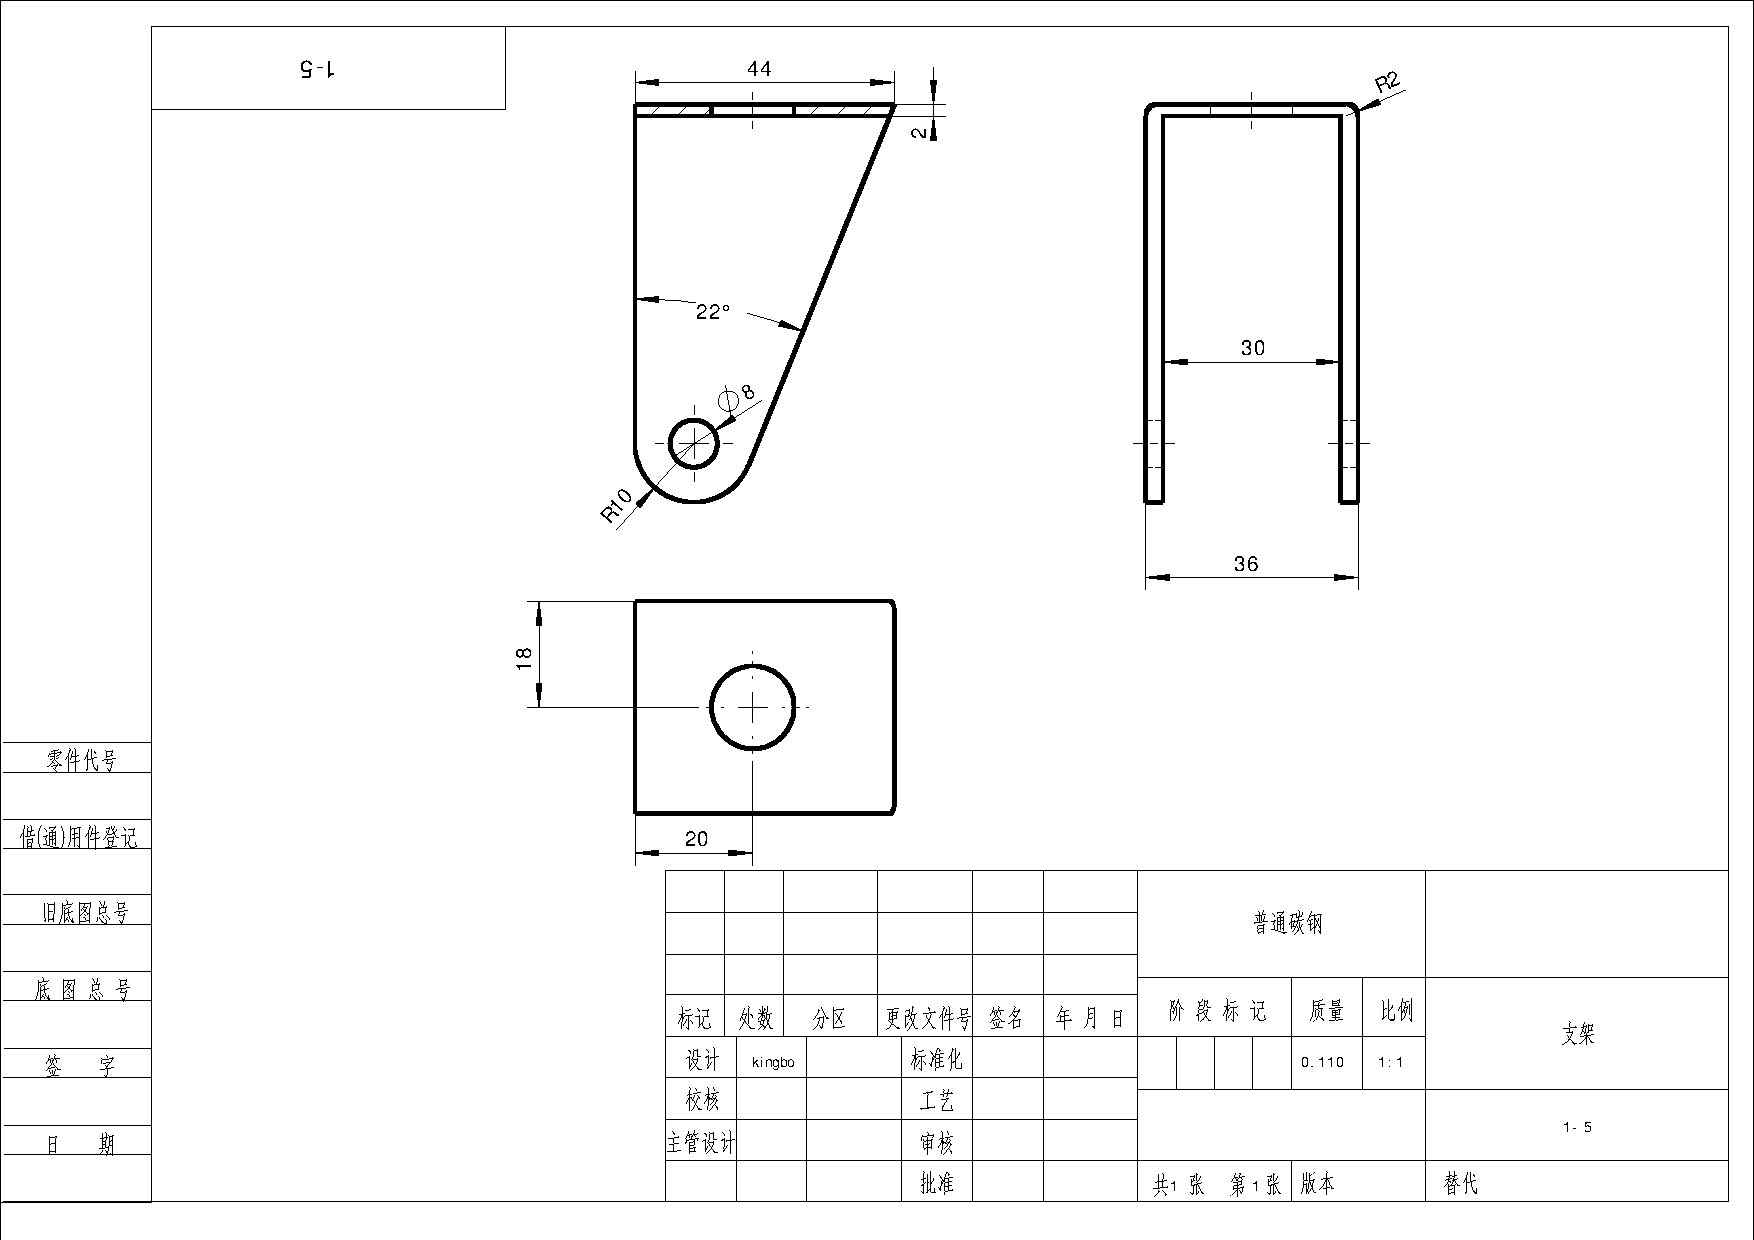
\includegraphics[scale=0.45]{xiaolunzhijia.pdf}
\caption{支架零件图}\label{fig:xiaolunzhijia}
\end{figure}

本章的目标是构建图\ref{fig:xiaolunzhijia}所示的小轮组支架零件的三维模型,并在此基础之上制作支架的三视图。因此本章重点讲解以下内容:
\begin{itemize}
\item 支架的三维模型构建
\item 支架三视图的制作
\end{itemize}

\section{支架三维建模分析}

\subsection{切割法建模}
所谓切割法是从具备包容待建模模型基本形体之中逐步切除多余部分,从而实现三维模型构构建的方法。图\ref{fig:zhijiafenxi0}为构建支架模型的基本楔体,在此基础之上去除圆角之外多余部分材料构成图\ref{fig:zhijiafenxi1}的结果,图\ref{fig:zhijiafenxi2}是去除孔材料的结果,图\ref{fig:zhijiafenxi3}是去除中间部分多余材料的结果。其整个过程是不断的切除多余的材料来实现支架模型。

\begin{figure}[htbp]
\centering
\subfloat[]{\label{fig:zhijiafenxi0}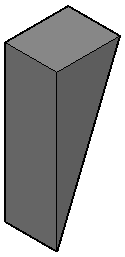
\includegraphics[scale=0.5]{zhijiafenxi0}}\hspace{20pt}
\subfloat[]{\label{fig:zhijiafenxi1}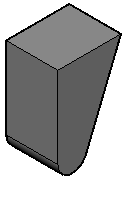
\includegraphics[scale=0.5]{zhijiafenxi1}}\hspace{20pt}
\subfloat[]{\label{fig:zhijiafenxi2}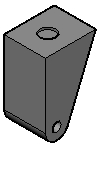
\includegraphics[scale=0.6]{zhijiafenxi2}}\hspace{20pt}
\subfloat[]{\label{fig:zhijiafenxi3}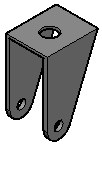
\includegraphics[scale=0.6]{zhijiafenxi3}}
\caption{切割法建模支架}
\end{figure}

\subsection{叠加法建模}

所谓叠加法是将待建模的形体切割为多个组成部分,然后将各个组成部分叠加组合在一起来构建三维模型的建模方法。图\ref{fig:zhijiafenxi4}的平板和图\ref{fig:zhijiafenxi5}的支耳是支架的基本组成部分,将两部分有效的组合在一起即可构建图\ref{fig:zhijiafenxi6}所示的支架三维模型。

\begin{figure}[htbp]
\centering
\subfloat[]{\label{fig:zhijiafenxi4}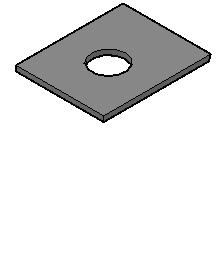
\includegraphics[scale=0.5]{zhijiafenxi4}}\hspace{20pt}
\subfloat[]{\label{fig:zhijiafenxi5}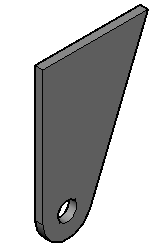
\includegraphics[scale=0.5]{zhijiafenxi5}}\hspace{20pt}
\subfloat[]{\label{fig:zhijiafenxi6}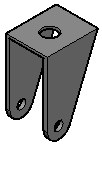
\includegraphics[scale=0.9]{zhijiafenxi3}}
\caption{叠加法建模支架}
\end{figure}

在实际的模型构建过程中经常需要将叠加建模法和切割建模法组合起来运用,如图\ref{fig:zhijiafenxi4}的平板和图\ref{fig:zhijiafenxi5}的支耳中的孔是运用切割法来完成。

\endinput
\section{支架三维建模}

切割建模法和叠加建模法不仅适用于实体建模,也适用于采用旋转和拉伸方式构建三维模型。切割建模法和叠加建模法是通用性的方法。本节将采用叠加建模法来构建支架的三维模型。

\subsection{构建顶板}
\begin{procedure}
\item 切换视图方向为西南等轴测

\begin{lstlisting}
命令: -VIEW
输入选项 [?/删除(D)/正交(O)/恢复(R)/保存(S)/设置(E)/窗口(W)]: swiso
\end{lstlisting}

\item 构建顶板基础

忽略顶板的倒角和孔后,其视图所表达的是一长方体。长方体是一种基本几何体,它属于平面立体中的直棱柱。所谓平面立体是指立体表面均由平面构成。在平面立体中,平面立体的表面是由若干个平面多边形构成的,多边形的边是平面立体的轮廓线,也是平面立体两个平面的交线,当轮廓的投影可见时,用粗实线表示;不可见时,用虚线表示;当实线与虚线重合时,应当用粗实线表示。棱柱体通常由顶面、底面及若干个侧棱面构成。棱柱体的各个侧棱相互平行,顶面和底面相互平行。如果棱柱的侧棱与顶面和底面垂直则称为直棱柱,否则称为斜棱柱。当直棱柱的顶面和底面为正多边形时则称为正棱柱。图\ref{fig:cube}和图\ref{fig:cubethreeview}分别为长方体的立体图和三视图。从图\ref{fig:cubethreeview}中可知,长方体的顶面与底面的水平投影重合并反映实形,为一长方形,其它棱面的水平投影积聚为长方形的四条边;前面与后面的正投影重合并反映实形,顶面、底面和两个侧面积聚为长方形的四条件边;左面和右面的侧面投影重合并反映实形,顶面、底面、前面和后面积聚为长方形的四条件边。

\begin{figure}[htbp]
\centering
\subfloat[]{\label{fig:cube}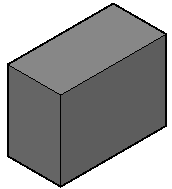
\includegraphics[scale=0.9]{cube.png}}\hspace{30pt}
\subfloat[]{\label{fig:cubethreeview}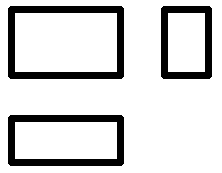
\includegraphics[scale=1]{cubethreeview.png}}
\caption{长方体的投影}
\end{figure}

因此构建长方体作为顶板建模的基础是比较方便快捷的。在AutoCAD中,调用绘制长方体命令的方法有:
\begin{itemize}
\item 键盘输入box\index{box,长方体}
\item 【绘图】$\rightarrow $【建模】$\rightarrow $【长方体】
\item 【实体】
\includegraphics[scale=0.45]{solidtoolbar}工具栏中的【长方体】
\includegraphics[scale=0.45]{boxtool}图标
\end{itemize}

调用长方体命令后,命令提示指定第一外角点,此时用鼠标在三维空间中任意指定一点。
\begin{lstlisting}
命令: BOX
指定第一个角点或 [中心(C)]:
\end{lstlisting}

接下来,参照支架零件图中的尺寸以相对坐指定另一个角点。
\begin{lstlisting}
指定其他角点或 [立方体(C)/长度(L)]: @44,36
\end{lstlisting}

然后,依据零件图中的尺寸指定支架顶板的高度,结果如图\ref{fig:zhijiajianmo1}所示。

\begin{lstlisting}
指定高度或 [两点(2P)]: 2
\end{lstlisting}

\begin{figure}[htbp]
\centering
\begin{floatrow}[2]
\ffigbox{\caption{顶板基础}\label{fig:zhijiajianmo1}}{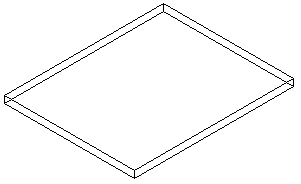
\includegraphics[scale=0.7]{zhijiajianmo1}}
\ffigbox{\caption{三点创建UCS}}{
\subfloat[]{\label{fig:ucsselectnode1}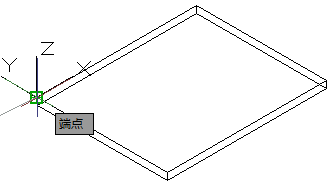
\includegraphics[scale=0.3]{ucsselectnode1}}\hspace{20pt}
\subfloat[]{\label{fig:ucsselectnode2}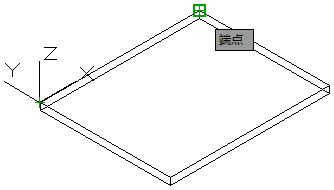
\includegraphics[scale=0.3]{ucsselectnode2}}\\
\subfloat[]{\label{fig:ucsselectnode3}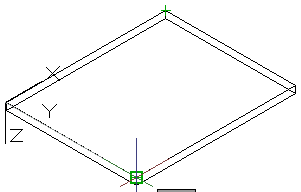
\includegraphics[scale=0.3]{ucsselectnode3}}\hspace{20pt}
\subfloat[]{\label{fig:zhijiajianmo2}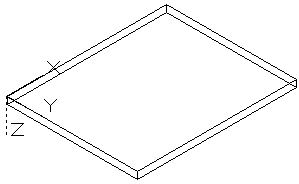
\includegraphics[scale=0.3]{zhijiajianmo2}}
}
\end{floatrow}
\end{figure}

\item 制作顶板孔

\begin{enumerate}
\item 切换用户坐标系

为方便制作支架顶板上的孔,我们将用户坐标系定义到顶板的角点上,其操作方法是采用默认的三点方式,即按图\ref{fig:ucsselectnode1}的方式指定原点,按图\ref{fig:ucsselectnode2}的方式指定$x$轴上的点,按图\ref{fig:ucsselectnode3}的方式指定$y$轴上的点,最终的坐标系效果如图\ref{fig:zhijiajianmo2}所示。从图中可以看出,$z$轴的正方向是指向俯视投影面的。


\begin{lstlisting}
命令: UCS
当前 UCS 名称: *世界*
指定 UCS 的原点或 [面(F)/命名(NA)/对象(OB)/上一个(P)/视图(V)/世界(W)/X/Y/Z/Z 轴(ZA)] <世界>:
指定 X 轴上的点或 <接受>:
指定 XY 平面上的点或 <接受>:
\end{lstlisting}


\item 绘制孔圆柱体

由于用户坐标系已经移动到长方体的角点之上,因此可根据支架零件图中的定圆心定位尺寸用绝对坐标来指定圆柱体的底圆圆心。

\begin{lstlisting}
命令: CYLINDER
指定底面的中心点或 [三点(3P)/两点(2P)/切点、切点、半径(T)/椭圆(E)]: 20,18
指定底面半径或 [直径(D)]: 7
指定高度或 [两点(2P)/轴端点(A)] <2.0000>: 2
\end{lstlisting}

\yaodian{适时的切换用户坐标系能够利用更方便的定位。}

\item 做差集

完成差集操作后,顶板孔的效果如图\ref{fig:zhijiajianmo3}所示。
\begin{lstlisting}
命令: SUBTRACT 
选择要从中减去的实体、曲面和面域...
选择对象: 找到 1 个
选择对象:  选择要减去的实体、曲面和面域...
选择对象: 找到 1 个
选择对象:
\end{lstlisting}

\end{enumerate}

\begin{figure}[htbp]
\centering
\begin{floatrow}[2]
\ffigbox{\caption{制作顶板孔}\label{fig:zhijiajianmo3}}{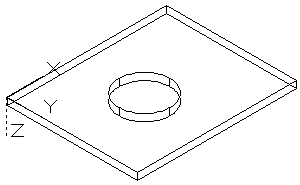
\includegraphics[scale=0.7]{zhijiajianmo3}}
\ffigbox{\caption{制作倒角边}\label{fig:zhijiajianmo4}}{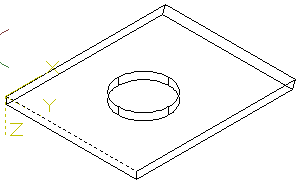
\includegraphics[scale=0.7]{zhijiajianmo4}}
\end{floatrow}
\end{figure}
\item 倒角边

根据支架零件图可知顶板的上的倒角边是整个面斜斜22度,由于倒角边命令不具备指定角度的功能。因此需要通过三角函数计算另一边的长度才能够准确地倒出22度的倒角边。直接用计算器计算出准确的值后输入的方法虽然能够完成,但这样做并不可取。主要是因为AutoCAD本身就具备计算功能,可以轻松地完成此类计算,故选择[表达式(E)]选项,并输入正确的计算表达式。顶板倒角边后的效果如图\ref{fig:zhijiajianmo4}所示。


\begin{lstlisting}
命令: CHAMFEREDGE
距离 1 = 1.0000,距离 2 = 1.0000
选择一条边或 [环(L)/距离(D)]: d
指定距离 1 或 [表达式(E)] <1.0000>: 2
指定距离 2 或 [表达式(E)] <1.0000>: e
输入表达式: 2*tan(22)
选择一条边或 [环(L)/距离(D)]:
选择同一个面上的其他边或 [环(L)/距离(D)]:
按 Enter 键接受倒角或 [距离(D)]:
\end{lstlisting}

\end{procedure}

\subsection{构建支耳}
\begin{procedure}
\item 制作支耳基础楔体

支架支耳忽略倒圆角后可以简化为一个基本的楔体。在AutoCAD中构建楔体命令的调用方法有:
\begin{itemize}
\item 键盘输入wedge\index{wedge,楔体}
\item 【绘图】$\rightarrow $【建模】$\rightarrow $【楔体】
\item 【实体】
\includegraphics[scale=0.45]{solidtoolbar} 工具栏中的【楔体】
\includegraphics[scale=0.45]{wedgetool}图标
\end{itemize}

楔体命令调用后以需要指定两个对角点来绘制底面,此操作与长方体定义底面的操作是一致的。此时在顶板的旁边任意点取一点来指定第一个角点,然后根据尺寸用相对坐标指定第二个角点。

\begin{lstlisting}
命令: wedge
指定第一个角点或 [中心(C)]:
指定其他角点或 [立方体(C)/长度(L)]: @44,3
\end{lstlisting}

接下来需要指定楔体的高度,由于无法从零件图中直接获取高度尺寸,因此也需要通过计算来获取高度值。但是楔体命令没有表达式选项,如何才能够使用AutoCAD的计算功能呢?其方法是调用计算器命令,即在命令行中输入\lstinline{'cal} \index{cal,计算器}来临时调用计算器,然后输入表达式进行计算。最终结果如图\ref{fig:zhijiajianmo5}所示。
\begin{lstlisting}
指定高度或 [两点(2P)] <2.0000>: 'cal
>>>> 表达式: 44/tang(22)
正在恢复执行 WEDGE 命令。
指定高度或 [两点(2P)] <2.0000>: 108.90382155032
\end{lstlisting}

\begin{figure}[htbp]
\centering
\begin{floatrow}[3]
\ffigbox{\caption{支耳基础楔体}\label{fig:zhijiajianmo5}}{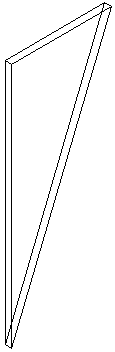
\includegraphics[scale=0.4]{zhijiajianmo5}}
\ffigbox{\caption{楔体倒圆角}\label{fig:zhijiajianmo6}}{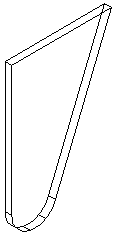
\includegraphics[scale=0.6]{zhijiajianmo6}}
\ffigbox{\caption{构建支耳孔}\label{fig:zhijiajianmo7}}{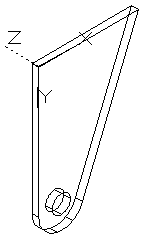
\includegraphics[scale=0.6]{zhijiajianmo7}}
\end{floatrow}
\end{figure}
\item 倒支耳圆角边

接下来,用圆角边命令制作$R10$的圆角边,效果如图\ref{fig:zhijiajianmo6}所示。

\begin{lstlisting}
命令: FILLETEDGE
半径 = 1.0000
选择边或 [链(C)/环(L)/半径(R)]: r
输入圆角半径或 [表达式(E)] <1.0000>: 10
选择边或 [链(C)/环(L)/半径(R)]:
选择边或 [链(C)/环(L)/半径(R)]:
已选定 1 个边用于圆角。
按 Enter 键接受圆角或 [半径(R)]:
\end{lstlisting}

\item 制作孔

\begin{enumerate}
\item 切换用户坐标系

由于AutoCAD中圆柱体底面是与$XY$平面平行的,而支耳中的圆柱孔的底面是与主视图平行的,因此需要切换用用户坐标系,使用户坐标系中的$XY$平面与主视图平行。

\begin{lstlisting}
命令: UCS
当前 UCS 名称: *没有名称*
指定 UCS 的原点或 [面(F)/命名(NA)/对象(OB)/上一个(P)/视图(V)/世界(W)/X/Y/Z/Z 轴(ZA)] <世界>:
指定 X 轴上的点或 <接受>:
指定 XY 平面上的点或 <接受>:
\end{lstlisting}

\yaodian{理解AutoCAD基本实体与$XY$平面之间的关系,能够有助于建立更有针对性的用户坐标系。}

\item 构建孔圆柱体

以支耳的圆角边的前圆心做为孔圆柱体的底圆圆心来构建孔圆柱体。
\begin{lstlisting}
命令: CYLINDER
指定底面的中心点或 [三点(3P)/两点(2P)/切点、切点、半径(T)/椭圆(E)]:
指定底面半径或 [直径(D)] <7.0000>: 4
指定高度或 [两点(2P)/轴端点(A)] <108.9038>: 3
\end{lstlisting}

\item 做差集

然后,从支耳中去除孔的圆柱体便可得到支耳的孔,效果如图\ref{fig:zhijiajianmo7} 所示。
\begin{lstlisting}
命令: SUBTRACT 
选择要从中减去的实体、曲面和面域...
选择对象: 找到 1 个
选择对象:  选择要减去的实体、曲面和面域...
选择对象: 找到 1 个
选择对象:
\end{lstlisting}

\end{enumerate}
\end{procedure}

\subsection{组合构建支架}
\begin{procedure}
\item 叠加支耳

由于顶板和支耳是分别制作的,故需要将两者组合起来构成一个整个。因此需要将支耳叠加到顶板之上;当然也可以将顶板叠加在支耳之上,两者效果是一样的。在AutoCAD中实现两对象叠加命令有移动和三维对齐。移命令只能用于已经建立的模型组件与实际需要方向一致的情况,三维对齐命令不仅能够适用于方向一致的情况,也适用于不一致的情况。当模型组件与实际方向一致时,使用移动命令则最为简便。AutoCAD中调用移动命令的方法有:
\begin{itemize}
\item 键盘输入move\index{move,移动}或M
\item 【修改】$\rightarrow $【移动】
\item 【修改】
\includegraphics[scale=0.45]{edittools}工具栏中的【移动】
\includegraphics[scale=0.45]{movetool}图标
\end{itemize}

\begin{figure}[htbp]
\centering
\subfloat[]{\label{fig:moveselectobj}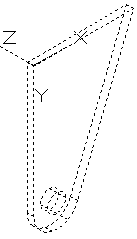
\includegraphics[scale=0.5]{moveselectobj}}\hspace{20pt}
\subfloat[]{\label{fig:moveselectbase}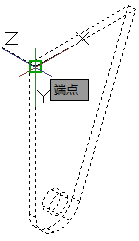
\includegraphics[scale=0.5]{moveselectbase}}\hspace{20pt}
\subfloat[]{\label{fig:moveselectsec}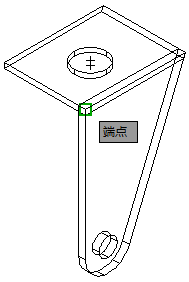
\includegraphics[scale=0.5]{moveselectsec}}\hspace{20pt}
\subfloat[]{\label{fig:moveresult}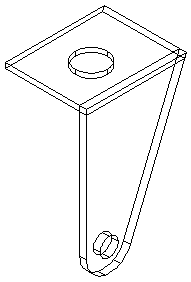
\includegraphics[scale=0.5]{moveresult}}
\caption{移动操作过程}
\end{figure}

调用移动命令后,会提示选择要移动的对象,此时用鼠标选择支耳作为要移动的对象,选择后会以虚线形式显示,效果如图\ref{fig:moveselectobj}所示。

\begin{lstlisting}
命令: MOVE
选择对象: 找到 1 个
选择对象:
\end{lstlisting}

接下来选择图\ref{fig:moveselectbase}所示的点作为基点。

\begin{lstlisting}
指定基点或 [位移(D)] <位移>:
\end{lstlisting}

最后选择图\ref{fig:moveselectsec}所示的点作为第二点,操作完成后即可支耳移动到顶板之上,效果如图\ref{fig:moveresult}所示。

\begin{lstlisting}
指定第二个点或 <使用第一个点作为位移>:
\end{lstlisting}

\item 制作支耳镜像

支架具有两个支耳,因此需要使用镜像的方法直接生成另一个支耳,在本例中将使用三点方式来指定镜像面。即选择图\ref{fig:mirror3dselectnode1}所示中点作为镜像平面上的第一点,选择图\ref{fig:mirror3dselectnode2}所示中点作为镜像平面上的第二点,选择图\ref{fig:mirror3dselectnode3}所示中点作为镜像平面上的第三点。完成后效果如图\ref{fig:zhijiajianmo8}所示。

\begin{figure}[htbp]
\centering
\subfloat[]{\label{fig:mirror3dselectnode1}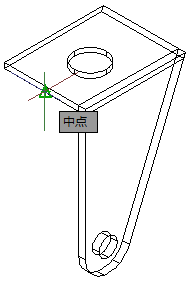
\includegraphics[scale=0.5]{mirror3dselectnode1}}\hspace{20pt}
\subfloat[]{\label{fig:mirror3dselectnode2}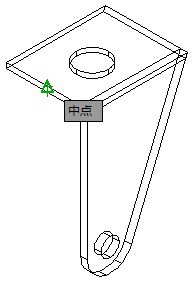
\includegraphics[scale=0.5]{mirror3dselectnode2}}\hspace{20pt}
\subfloat[]{\label{fig:mirror3dselectnode3}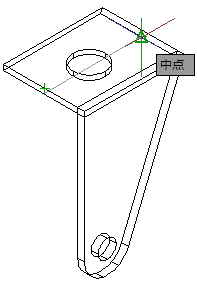
\includegraphics[scale=0.5]{mirror3dselectnode3}}\hspace{20pt}
\subfloat[]{\label{fig:zhijiajianmo8}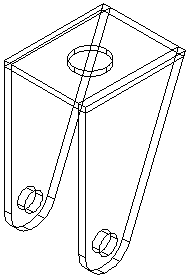
\includegraphics[scale=0.5]{zhijiajianmo8}}
\end{figure}

\begin{lstlisting}
命令: MIRROR3D
选择对象: 找到 1 个
选择对象:
指定镜像平面 (三点) 的第一个点或
  [对象(O)/最近的(L)/Z 轴(Z)/视图(V)/XY 平面(XY)/YZ 平面(YZ)/ZX 平面(ZX)/三点(3)] <三点>: 
  在镜像平面上指定第二点: 
  在镜像平面上指定第三点:
是否删除源对象?[是(Y)/否(N)] <否>:
\end{lstlisting}

\item 合并实体

接下来将顶板和两个支耳组合在一起,形成一个整个体,为另外两圆边创造条件。

\begin{lstlisting}
命令: UNION
选择对象: 指定对角点: 找到 3 个
选择对象:
\end{lstlisting}

\item 倒圆角边

完成合并操作后,需要构建支架中两个$R2$圆角边的才能够最终完成支架的建模,完成后效果如图\ref{fig:zhijiajianmo9}所示。

\begin{lstlisting}
命令: FILLETEDGE
半径 = 10.0000
选择边或 [链(C)/环(L)/半径(R)]: r
输入圆角半径或 [表达式(E)] <10.0000>: 2
选择边或 [链(C)/环(L)/半径(R)]:
选择边或 [链(C)/环(L)/半径(R)]:
选择边或 [链(C)/环(L)/半径(R)]:
已选定 2 个边用于圆角。
按 Enter 键接受圆角或 [半径(R)]:
\end{lstlisting}

\begin{figure}[htbp]
\centering
\begin{floatrow}[2]
\ffigbox{\caption{支架倒圆角}\label{fig:zhijiajianmo9}}{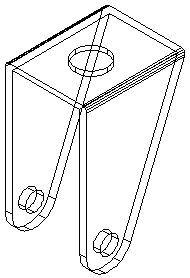
\includegraphics[scale=0.5]{zhijiajianmo9}}
\ffigbox{\caption{支架三维模型}\label{fig:zhijiajianmo10}}{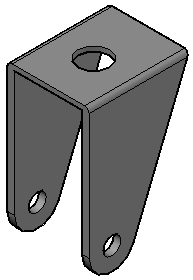
\includegraphics[scale=0.5]{zhijiajianmo10}}
\end{floatrow}
\end{figure}
\item 切换视觉样式为灰度


\begin{lstlisting}
命令: VSCURRENT
输入选项 [二维线框(2)/线框(W)/隐藏(H)/真实(R)/概念(C)/着色(S)/带边缘着色(E)/灰度(G)/勾画(SK)/X 射线(X)/其他(O)] <二维线框>: g
\end{lstlisting}

将视觉样式切换为灰度后,最终的支架三维模型效果如图\ref{fig:zhijiajianmo10}所示。
\item 保存支架模型

最后将建立的支架三维模型以“支架.dwg”的文件名予以保存。

\end{procedure}

\endinput
\section{支架零件图制作}
\begin{procedure}

\begin{figure}[htbp]
\centering
\subfloat[]{\label{fig:layoutwizard1}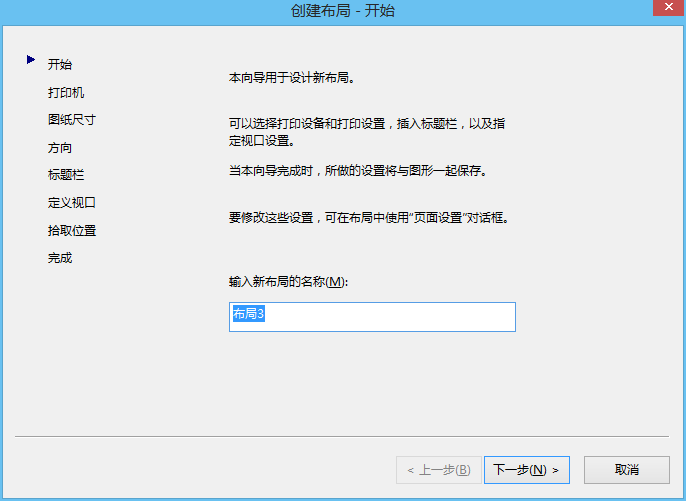
\includegraphics[scale=0.15]{layoutwizard1}}\hspace{20pt}
\subfloat[]{\label{fig:layoutwizard2}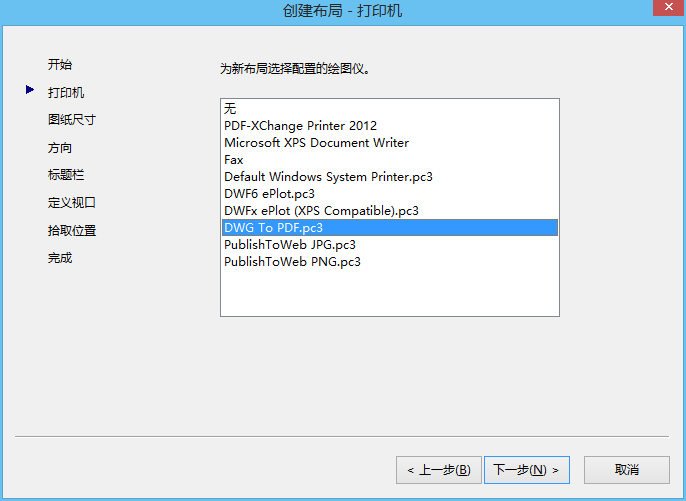
\includegraphics[scale=0.15]{layoutwizard2}}\hspace{20pt}
\subfloat[]{\label{fig:layoutwizard3}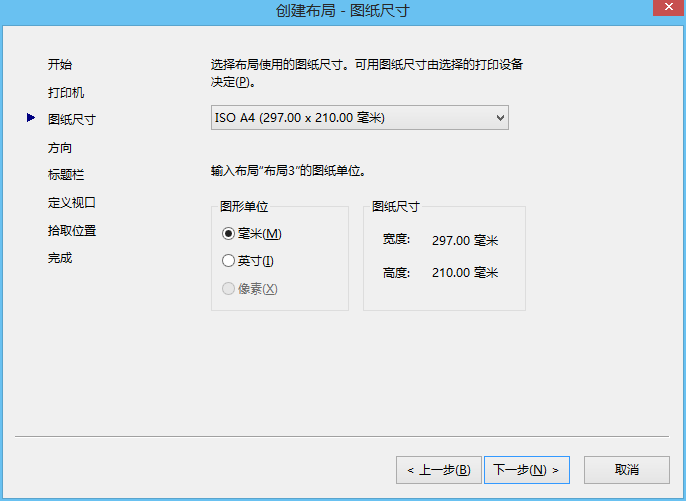
\includegraphics[scale=0.15]{layoutwizard3}}
\caption{新建布局过程(一)}
\end{figure}

\item 创建新布局

由于系统创建的窗口布局通常是不能够满足实际布局需求的,为适应支架三视图生成的需要,我们可以采用新建布局向导来进行设置。AutoCAD中调用新建布局向导的方法有:
\begin{itemize}
\item 键盘输入layoutwizard\index{layoutwizard,创建布局向导}
\item 【插入】$\rightarrow $【布局】$\rightarrow $【创建布局向导】
\end{itemize}

调用布局向导命令会弹出图\ref{fig:layoutwizard1}所示的创建布局对话框,在文本框中输入新布局的名称;点击下一步进入图\ref{fig:layoutwizard2}所示的打印机设置步骤,将打印机设置为“DWG TO PDF.pc3”;点击下一步进入图\ref{fig:layoutwizard3}所示的图纸尺寸设置步骤,将图纸尺寸设置为“ISO A4(297.00x210.00毫米)";点击下步进入图\ref{fig:layoutwizard4}所示的方向设置步骤,由于A4图纸比较小,对放置三视图而言设置为纵向比较合理,故选择纵向;点击下一下进入图\ref{fig:layoutwizard5}所示的标题栏设置步骤,由于无符合国家标准的标题栏,故选择无;点击下一步进入图\ref{fig:layoutwizard6}所示的定义视口步骤,为方便后续操作,将其设置为无视口;点击下一步进入图\ref{fig:layoutwizard7}完成布局创建。

\begin{figure}[htbp]
\centering
\subfloat[]{\label{fig:layoutwizard4}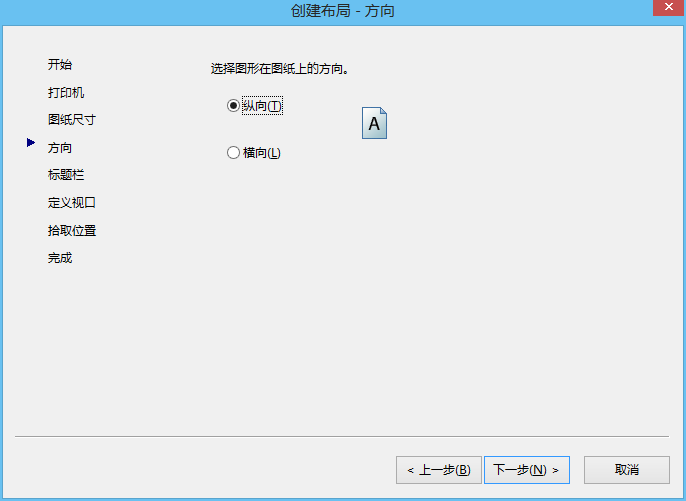
\includegraphics[scale=0.15]{layoutwizard4}}\hspace{20pt}
\subfloat[]{\label{fig:layoutwizard5}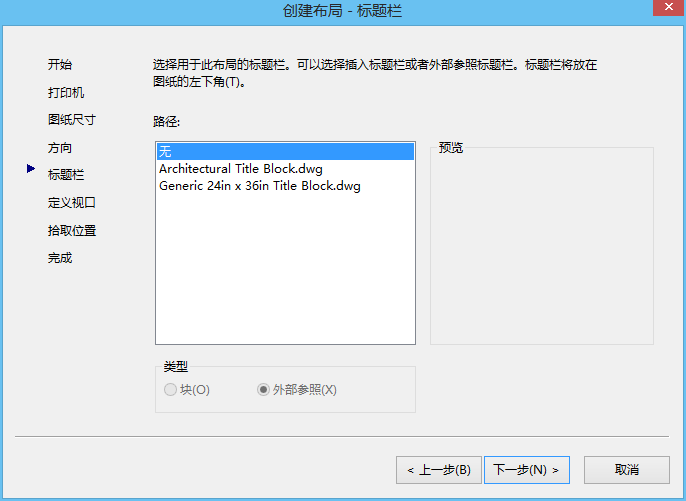
\includegraphics[scale=0.15]{layoutwizard5}}\hspace{20pt}
\subfloat[]{\label{fig:layoutwizard6}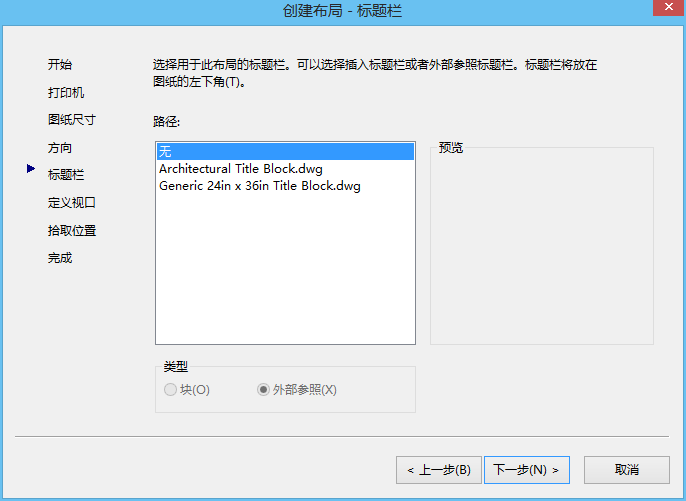
\includegraphics[scale=0.15]{layoutwizard5}}
\caption{新建布局过程(二)}
\end{figure}
\begin{lstlisting}
命令:LAYOUTWIZARD
\end{lstlisting}

\begin{figure}[htbp]
\centering
\subfloat[]{\label{fig:layoutwizard7}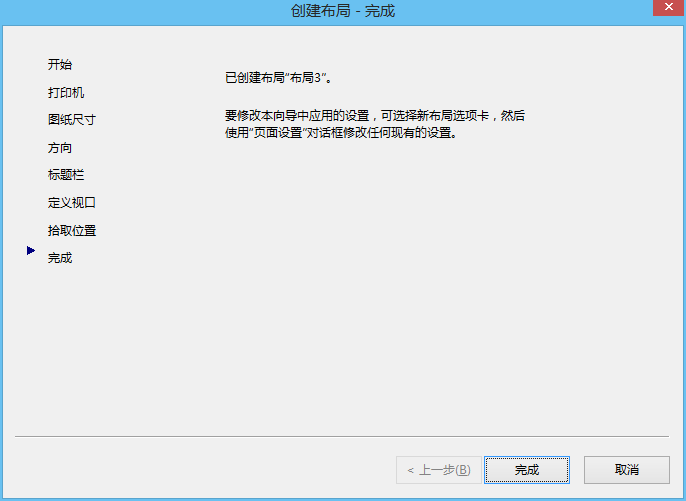
\includegraphics[scale=0.25]{layoutwizard7}}\hspace{20pt}
\subfloat[]{\label{fig:zhijiabuju1}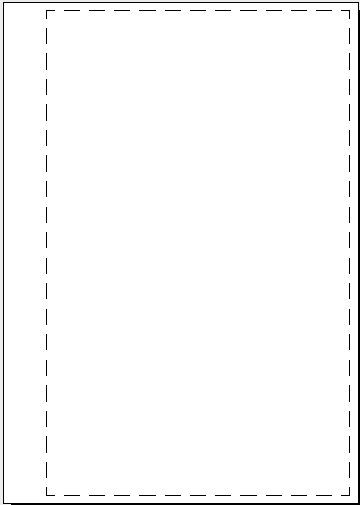
\includegraphics[scale=0.3]{zhijiabuju1}}
\caption{新建布局过程(三)}
\end{figure}

通过向导创建的布局其可打印区域通常不能够与标准图幅的要求是不一致的,因此需要利用页面设置管理器设置图纸可打印区域,最终结果如图\ref{fig:zhijiabuju1}所示。

\item 新建图层

新建“尺寸标注”和“标题栏”图层,线型为“continuous",线宽为默认;新建“中心线”图层,线型为“center",线宽为默认; 新建“图框”图层,线型为“continuous",线宽为0.5mm。

\item 制作图框与标题栏

设置当前图层为“图框”,绘制图框矩形。
\begin{lstlisting}
命令: RECTANG
指定第一个角点或 [倒角(C)/标高(E)/圆角(F)/厚度(T)/宽度(W)]: 0,0
指定另一个角点或 [面积(A)/尺寸(D)/旋转(R)]: @180,287
\end{lstlisting}

设置当前图层为“标题栏”,插入“GB标题栏”块。
\begin{lstlisting}
命令: INSERT
指定插入点或 [基点(B)/比例(S)/旋转(R)]:
\end{lstlisting}

\begin{figure}[htbp]
\centering

\end{figure}
\item 加载虚线线型

为方便于生成视图时系统自动设置虚线,需要先加载虚线线型。在AutoCAD中加载线型可调用线型管理器,其调用方式为:
\begin{itemize}
\item 键盘输入linetype\index{linetype}
\item 【格式】$\rightarrow $【线型】
\end{itemize}

调用线型管理器命令会弹出图\ref{fig:linetypemanarge}所示的对话框,点击加载按钮,并加载“HIDDEN”线型,结果如图\ref{fig:loadhiddenline}所示。

\begin{figure}[htbp]
\centering
\subfloat[]{\label{fig:linetypemanarge}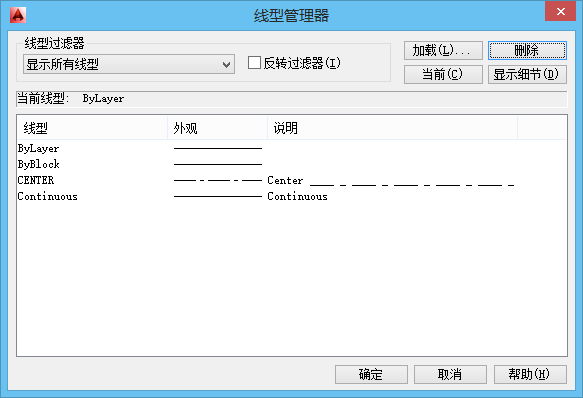
\includegraphics[scale=0.35]{linetypemanarge}}\hspace{20pt}
\subfloat[]{\label{fig:loadhiddenline}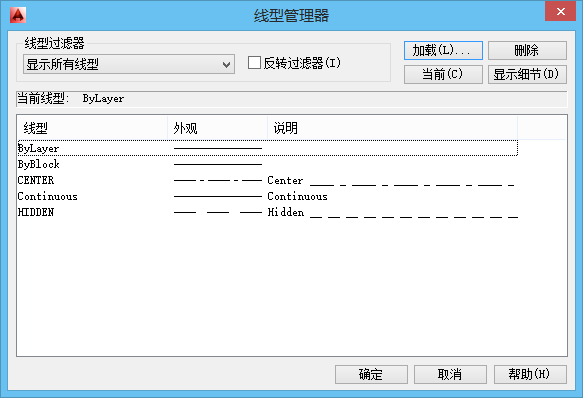
\includegraphics[scale=0.35]{loadhiddenline}}
\caption{线型管理}
\end{figure}

\begin{lstlisting}
命令: LINETYPE
\end{lstlisting}

\item 生成左视图

\begin{enumerate}
\item 新建左视图视口。

\begin{lstlisting}
命令: -VPORTS
指定视口的角点或 [开(ON)/关(OFF)/布满(F)/着色打印(S)/锁定(L)/对象(O)/多边形(P)/恢复(R)/图层(LA)/2/3/4] <布满>:
指定对角点:
\end{lstlisting}

\item 设置左视同图视口模型空间的视图方向为左视。
\begin{lstlisting}
命令: -VIEW
输入选项 [?/删除(D)/正交(O)/恢复(R)/保存(S)/设置(E)/窗口(W)]: left
\end{lstlisting}

\item 设置视口显示比例为1:1,结果如图\ref{fig:zhijiabuju3} 所示。

\end{enumerate}

\begin{figure}[htbp]
\centering
\begin{floatrow}[3]
\ffigbox[\FBwidth]{\caption{创建支架左视图显示}\label{fig:zhijiabuju3}}{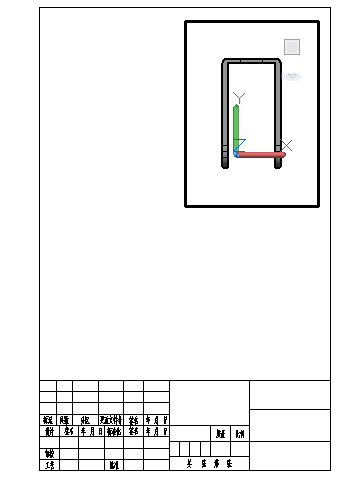
\includegraphics[scale=0.35]{zhijiabuju3}}
\ffigbox[\FBwidth]{\caption{创建支架主视图显示}\label{fig:zhijiabuju4}}{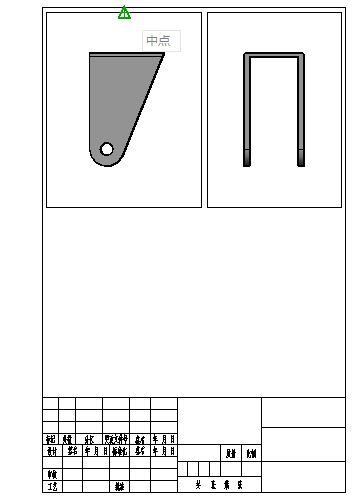
\includegraphics[scale=0.35]{zhijiabuju4}}
\ffigbox[\FBwidth]{\caption{创建支架俯视图显示}\label{fig:zhijiabuju5}}{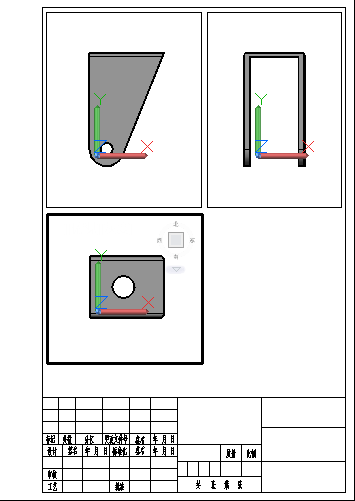
\includegraphics[scale=0.35]{zhijiabuju5}}
\end{floatrow}
\end{figure}

\item 生成全剖主视图

为更清楚地表达支架的内部结构,故采用全剖视图作为支架的主视图,能够实现既清楚表达支耳的结构又清楚表达顶板的孔。生成主视图的效果如图\ref{fig:zhijiabuju4}所示。

\begin{lstlisting}
命令: SOLVIEW
输入选项 [UCS(U)/正交(O)/辅助(A)/截面(S)]: s
指定剪切平面的第一个点:
指定剪切平面的第二个点:
指定要从哪侧查看:
输入视图比例 <1>:
指定视图中心:
指定视图中心 <指定视口>:
指定视口的第一个角点: 
指定视口的对角点:
输入视图名: front
输入选项 [UCS(U)/正交(O)/辅助(A)/截面(S)]:
\end{lstlisting}


\item 生成俯视图

双击进入主视图所在的视口模型空间,然后以主视图为基础用正交选项生成普通的俯视图,结果如图\ref{fig:zhijiabuju5}所示。

\begin{lstlisting}
命令: SOLVIEW
输入选项 [UCS(U)/正交(O)/辅助(A)/截面(S)]: o
指定视口要投影的那一侧:
指定视图中心:
指定视图中心 <指定视口>:
指定视口的第一个角点:
指定视口的对角点:
输入视图名: top
输入选项 [UCS(U)/正交(O)/辅助(A)/截面(S)]:
\end{lstlisting}

\item 生成左视图轮廓

到目前为止,还没有生成左视图。由于左视图是生成主视图的基础,因此只能用轮廓命令生成左视图。

\begin{lstlisting}
命令: SOLPROF
选择对象: 找到 1 个
选择对象:
是否在单独的图层中显示隐藏的轮廓线?[是(Y)/否(N)] <是>:
是否将轮廓线投影到平面?[是(Y)/否(N)] <是>:
是否删除相切的边? [是(Y)/否(N)] <是>:
\end{lstlisting}

\item 图形化主视图和俯视图

\begin{figure}[htbp]
\centering
\subfloat[]{\label{fig:zhijiabuju6}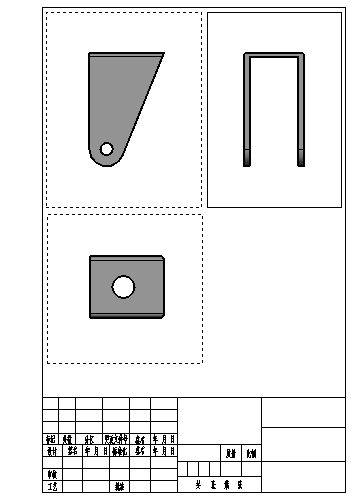
\includegraphics[scale=0.4]{zhijiabuju6}}\hspace{20pt}
\subfloat[]{\label{fig:zhijiabuju7}\includegraphics[scale=0.4]{zhijiabuju7}}
\caption{生成最终主俯视图}
\end{figure} 

选择主视图和俯视图作为图形化对象,选择后的效果如图\ref{fig:zhijiabuju6}所示。

\begin{lstlisting}
命令: SOLDRAW
选择要绘图的视口...
选择对象: 找到 1 个
选择对象: 找到 1 个,总计 2 个
选择对象:
\end{lstlisting}

\item 修改主视图图案填充

由于主视图的图案填充不符合国家标准的要求,故用图案填充编辑命令将填充图案修改为ANSI31。最终主视图和俯视图效果如图\ref{fig:zhijiabuju7}所示。

\begin{lstlisting}
命令: HATCHEDIT
选择图案填充对象:
\end{lstlisting}

\item 设置图层

按图\ref{fig:zhijiabuju8}进行支架的图层设置。
\begin{figure}[htbp]
\centering
\begin{floatrow}[2]
\ffigbox{\caption{支架图层设置}\label{fig:zhijiabuju8}}{\includegraphics[scale=0.35]{zhijiabuju8}}
\ffigbox{\caption{绘制中心线结果}\label{fig:zhijiabuju9}}{\includegraphics[scale=0.35]{zhijiabuju9}}
\end{floatrow}
\end{figure}
\item 绘制中心线

将当前图层设置为“中心线”图层,并绘制支架孔的中心线,结果如图\ref{fig:zhijiabuju9}所示。

\item 标注尺寸
\begin{enumerate}
\item 设置标注样式

按\ref{sec:lianjieganshitu}节的步骤设置标注样式。

\item 标注线性尺寸

完成支架三视图中所有线性尺寸的标注,结果如图\ref{fig:zhijiabuju10} 所示。

\begin{figure}[htbp]
\centering
\subfloat[]{\label{fig:zhijiabuju10}\includegraphics[scale=0.2]{zhijiabuju10}}\hspace{20pt}
\subfloat[]{\label{fig:zhijiabuju11}\includegraphics[scale=0.2]{zhijiabuju11}}\hspace{20pt}
\subfloat[]{\label{fig:zhijiabuju12}\includegraphics[scale=0.2]{zhijiabuju12}}\hspace{20pt}
\subfloat[]{\label{fig:zhijiabuju13}\includegraphics[scale=0.2]{zhijiabuju13}}
\caption{支架尺寸标注}
\end{figure}

\item 标注半径尺寸

完成支架三视图中所有圆弧的半径尺寸标注,结果如图\ref{fig:zhijiabuju11}所示。

\item 标注直径尺寸

完成支架三视图中所有圆的直径尺寸标注,结果如图\ref{fig:zhijiabuju12}所示。
\item 标注角度尺寸

对于支架中的角度尺寸需要调用AutoCAD中的角度标注命令,其方法有:
\begin{itemize}
\item 键盘输入dimangular\index{dimanglar,角度标注}
\item 【标注】$\rightarrow $【角度】
\item 【标注】\includegraphics[scale=0.45]{dimtoolsbar}工具栏中的【角度】\includegraphics[scale=0.45]{dimangular}图标
\end{itemize}

调用角度标注命令后,选择两条直线并指定标注线的位置即可完成角度标注,其结果如图\ref{fig:zhijiabuju13}所示。

\begin{lstlisting}
命令: dimangular
选择圆弧、圆、直线或 <指定顶点>:
选择第二条直线:
指定标注弧线位置或 [多行文字(M)/文字(T)/角度(A)/象限点(Q)]:
标注文字 = 22
\end{lstlisting}

\end{enumerate}

\end{procedure}
\endinput

\endinput